\chapter{HGP-Clusterer : la généralisation du Single-Linkage dans l'espace euclidien} 
\label{chap:hgp_clusterer}
%\rouge{10 avril - 20 avril}

Ce chapitre commence par revenir sur le problème fondamental du Single-Linkage : l'effet de chaînage, ou la non prise en compte de la densité locale.
Si l'on voit -- ainsi que nous l'avons fait dans la partie précédente -- le Single-Linkage dans l'espace euclidien comme l'algorithme qui construit la hiérarchie exacte des amas de forte densité (modèle de \textsc{Hartigan}, voir \Def~\ref{def:high-density_clusters}~\&~\Def[def:HDC_discret]) pour l'estimateur de densité du $1$-NN, l'amélioration à apporter au Single-Linkage est claire :
\Citation{Il faut identifier la hiérarchie exacte des amas de forte densité pour l'estimateur de densité des $K$ plus proches voisins ($K$-NN).}

Nous verrons dans un premier temps (\S~\ref{sec:exemple_introductif}), sur un exemple simple, pourquoi les généralisations proposées au problème dans la partie précédente ne marchent pas. 
Comme nous l'avions déjà fait remarquer, le problème vient de ce que le Robust Single-Linkage \cite{RobustSingleLinkage2010} ou (H)DBSCAN \cite{HDBSCAN, HDBSCAN2017} imposent à un n\oe ud d'avoir $K$ voisins  (ou au moins d'être à la frontière de l'un de ces $K$-cœurs) pour apparaître au sein d'un cluster. Dans le même temps, une simple arête suffit pour connecter deux n\oe uds.
C'est cette asymétrie entre les contraintes (fortes) imposées aux points et celles (lâches) vis-à-vis des arêtes que nous allons réparer dans le présent chapitre.
Nous verrons alors toujours sur le même exemple la véritable solution au problème.

Nous passons alors à la formalisation de cette bonne réponse à apporter (\S~\ref{sec:KPolyedres}).
Des contraintes plus fortes (d'ordre supérieur) imposées aux liens peuvent être encodées en recourant aux hypergraphes, et plus particulièrement aux complexes simpliciaux \cite{Munkres}.
La réparation naturelle consiste à renforcer aussi la notion de ``connectivité''. 
Le bon objet à construire n'est plus le graphe géométrique, mais le complexe de \v Cech \cite{Cech1932, BobrowskiKahle} ; et la bonne notion de composante connexe n'est plus une composante de sommets reliés par des arêtes, mais une composante de $(K-1)$-simplexes reliés par des interactions d'ordre supérieur (ce que nous avons appelé des $K$-polyèdres).

En \S~\ref{sec:correspondance_KPolydres_KNN}, nous démontrons la correspondance exacte entre les $K$-polyèdres et les amas discrets de forte densité $K$-NN (\Th[th:cech_kpolyedres_knn]).

Nous ne chercherons pas ici à forcer une partition à chaque niveau. Pour $K\ge 2$, les amas discrets de forte densité (\Def[def:HDC_discret]) peuvent se recouvrir (\emph{cf}. l'exemple introductif en \S~\ref{sec:exemple_introductif}) ; la généralisation correcte du Single-Linkage doit donc produire, elle aussi, une hiérarchie de recouvrements (nous verrons au chapitre \ref{chap:conclusion_partie_II} comment faire pour obtenir une hiérarchie qui respecte strictement à tous niveaux la contrainte de partition).

À l'instar de la définition du Single-Linkage (\emph{via} l'analyse persistante de graphes géométriques, \emph{cf}. \Def[def:dendrogramme_gg]), la généralisation du Single-Linkage, que nous avons baptisée HGP-Clusterer (\Def[def:hgp_clusterer]), est pour l'instant toute théorique. Nous verrons au cours des chapitres suivants (dédiés à la généralisation et à la construction de l'arbre minimum couvrant) comment extraire cette hiérarchie en pratique.

\Contributions{Ce chapitre fait la transition entre la revue complète du Single-Linkage de la partie précédente, et la généralisation mathématiquement satisfaisante proposée. Nous espérons fournir au lecteur, \emph{via} la première section illustrative, la bonne intuition pour que cette généralisation lui paraisse effectivement naturelle. Les résultats présentés dans la suite du chapitre reprennent et reformulent \cite{BibiAppliedNetworkScience}. La reformulation adoptée dans ce manuscrit, plus naturelle et plus simple, a été permise grâce à notre définition d'un amas de forte densité $K$-NN \emph{discret} (\Def[def:HDC_discret]). Le résultat principal de ce chapitre est le \Th[th:cech_kpolyedres_knn], qui se montre sans difficulté une fois tous les bons outils introduits (amas discrets, régions témoins, graphe d'intersection, \emph{etc.}).}


\section{Retour sur la non prise en compte de la densité}
\label{sec:exemple_introductif}

\subsection{L'échec du Robust Single-Linkage et de (H)DBSCAN sur le modèle de \textsc{Hartigan}}

Appelons $K\in \mathbb N^\star$ la variable représentant le nombre de voisins pris en compte dans l'algorithme de Robust Single-Linkage \cite{RobustSingleLinkage2010} et de (H)DBSCAN \cite{HDBSCAN, HDBSCAN2017}.
Pour $K = 1$, l'on a vu que le Single-Linkage fournissait exactement la hiérarchie des amas de forte densité dans le modèle de \textsc{Hartigan}(voir la synthèse du chapitre \ref{chap:single-linkage_trois_vues}).

En revanche, pour $K\ge2$, il n'y a plus correspondance entre la hiérarchie produite par ces algorithmes et celle du modèle (discret) de \textsc{Hartigan}. 

Nous l'allons voir sur un exemple simple. Soit $\mathcal X = \bigl\{ A ; B ; C ; D ; E ; F\bigr\} \subset \mathbb R^2$ un nuage composé de six points disposés comme illustré en \Fig~\ref{fig:nuage} : deux triangles équilatéraux (de côté $2r$) parfaitement opposés et à distance $2r$ l'un de l'autre.


\begin{figure}[htbp]
    \centering
    
    % ---------------------------------------------------
    % SOUS-FIGURE (a) : Nuage de points X
    % ---------------------------------------------------
    \begin{subfigure}[b]{0.48\textwidth}
        \centering
        \begin{tikzpicture}[scale=0.6]
            
            % On définit le rayon r (la moitié de la longueur d'un segment)
            \def\r{1.5}
            
            % 1. Appel du template réutilisable
            \templateNuage[\r]
            
            % 2. Tracé des cercles en pointillés
            % (Les segments faisant 2r de long, les cercles sont magnifiquement 
            % tangents et se touchent au milieu parfait de chaque segment).
            \foreach \P in {A,B,C,D,E,F} {
                \draw[dashed, thick, gray] (\P) circle (\r);
            }
            
            % 3. Flèche pour faire apparaître visuellement le rayon r
            % On trace depuis A vers le haut-gauche (angle de 135 degrés).
            \draw[-, >=latex] (A) -- ++(135:\r) node[midway, sloped, above] {$r$};
            
        \end{tikzpicture}
        \caption{Niveau $r$}
        \label{fig:nuage}
    \end{subfigure}
    \hfill
    % ---------------------------------------------------
    % SOUS-FIGURE (b) : Dendrogramme sur X
    % ---------------------------------------------------
    \begin{subfigure}[b]{0.48\textwidth}
        \centering
        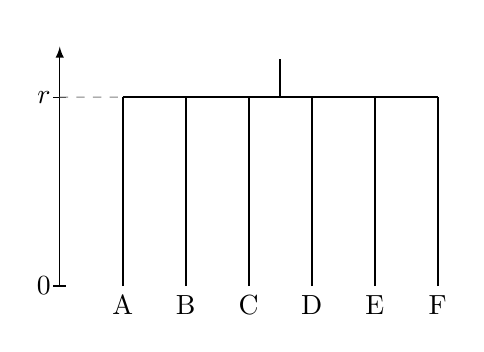
\begin{tikzpicture}[scale=0.8]
            
            % Les feuilles du dendrogramme (en bas de la figure)
            \coordinate (L1) at (0,0);
            \coordinate (L2) at (1,0);
            \coordinate (L3) at (2,0);
            \coordinate (L4) at (3,0);
            \coordinate (L5) at (4,0);
            \coordinate (L6) at (5,0);
            
            % Affichage des labels des 6 feuilles
            \node[below] at (L1) {A};
            \node[below] at (L2) {B};
            \node[below] at (L3) {C};
            \node[below] at (L4) {D};
            \node[below] at (L5) {E};
            \node[below] at (L6) {F};
            
            % Le niveau de fusion (haut) à la hauteur "h" qui symbolise le rayon "r"
            \def\h{3}
            \coordinate (T1) at (0,\h);
            \coordinate (T2) at (1,\h);
            \coordinate (T3) at (2,\h);
            \coordinate (T4) at (3,\h);
            \coordinate (T5) at (4,\h);
            \coordinate (T6) at (5,\h);
            
            % Lignes montantes (fusion 100% simultanée des 6 composantes)
            \draw[thick] (L1) -- (T1);
            \draw[thick] (L2) -- (T2);
            \draw[thick] (L3) -- (T3);
            \draw[thick] (L4) -- (T4);
            \draw[thick] (L5) -- (T5);
            \draw[thick] (L6) -- (T6);
            
            % Barre horizontale reliant toutes les branches
            \draw[thick] (T1) -- (T6);
            
            % Tige au-dessus de la fusion (racine de l'arbre)
            \draw[thick] (2.5, \h) -- (2.5, \h+0.6);
            
            % Axe vertical pour localiser clairement la valeur de la fusion (r)
            \draw[->, >=latex] (-1, 0) -- (-1, \h+0.8) node[above] {};
            \draw (-1.1, \h) -- (-0.9, \h) node[left=2pt] {$r$};
            \draw (-1.1, 0) -- (-0.9, 0) node[left=2pt] {$0$};
            \draw[dashed, gray] (-1, \h) -- (T1);
            
        \end{tikzpicture}
        \caption{Dendrogramme sur $\mathcal X$}
        \label{fig:dendrogramme}
    \end{subfigure}
    
    \caption{(Gauche) Nuage de six points $\mathcal X = \bigl\{A ; B ; C ; D ; E ; F\bigr\}$. (Droite) Dendrogramme produit par le Single-Linkage avec en entrée $\mathcal X$. Le même dendrogramme est produit par le Robust Single-Linkage et (H)DBSCAN pour $K=2$.}
    \label{fig:clustering}
\end{figure}

Chaque point a son plus proche voisin à distance $2r$. Mieux : pour ce seuil $2r$, chaque point a même au moins $K=2$ voisins. De plus, le graphe engendré par les connexions au seuil $2r$ connecte les six points de $\mathcal X$ entre eux. Il en résulte que le dendrogramme produit par le Robust Single-Linkage ou (H)DBSCAN avec $K=2$ est un arbre constitué de six feuilles (les six points de $\mathcal X$) qui fusionnent toutes au seuil $r$ (voir \Fig~\ref{fig:dendrogramme})\footnote{Ainsi d'ailleurs que le dendrogramme de (H)DBSCAN avec $K=3$, et aussi celui du Single-Linkage standard.}.

\subsection{La hiérarchie exacte de \textsc{Hartigan} lorsque $K=2$}

Calculons maintenant la hiérarchie (discrète) produite par le modèle de \textsc{Hartigan} lorsque $K=2$.
Rappelons (\Def[def:HDC_discret]) qu'un point $x\in\mathcal X$ est \emph{couvert} au niveau $r$ par un amas de forte densité $ C \in H_{\widehat f_K}(r)$ si $x $ est à moins de $r$ de $C$. On note $C^{\mathrm{discret}} \subseteq \mathcal X$ le cluster discret correspondant.


\begin{figure}[htbp]
    \centering
    
    % ---------------------------------------------------
    % SOUS-FIGURE (a) : Intersections pour r' > r
    % ---------------------------------------------------
    \begin{subfigure}[b]{0.45\textwidth}
        \centering
        \begin{tikzpicture}[scale=0.55]
            
            % r est la moitié du segment, r' est un peu plus grand
            \def\r{1.5}
            \def\rprime{1.60} 
            
            % 1. Appel du template (définit les points et trace le graphe principal)
            \templateNuage[\r]
            
            % 2. Dessin en arrière-plan pour ne rien cacher
            \begin{scope}[on background layer]
                
                % Remplissage bleu foncé des intersections deux à deux
                % La fonction \clip joue le rôle de pochoir : on se restreint au cercle \p
                % puis on dessine le cercle \q. Seule l'intersection apparaît !
                \foreach \p/\q in {A/B, B/C, C/A, C/D, D/E, E/F, F/D} {
                    \begin{scope}
                        \clip (\p) circle (\rprime);
                        \fill[blue!60!black, opacity=0.4] (\q) circle (\rprime);
                    \end{scope}
                }
                
                % Tracé des 6 cercles de rayon r' (en pointillés gris pour bien contraster avec le bleu)
                \foreach \P in {A,B,C,D,E,F} {
                    \draw[dashed, thick, gray!80] (\P) circle (\rprime);
                }
                
            \end{scope}
            
            % 3. Flèche pour indiquer le rayon r' (vers le haut pour ne pas traverser la lettre A)
            \draw[>=latex] (A) -- ++(120:\rprime) node[midway, sloped, above] {$r'$};
            
        \end{tikzpicture}
        \caption{Niveau $r' \gtrsim r$ et $2$-intersections en bleu.}
        \label{fig:intersections_rprime}
    \end{subfigure}
    \hfill
    % ---------------------------------------------------
    % SOUS-FIGURE (b) : Forêt de 7 dendrogrammes
    % ---------------------------------------------------
    \begin{subfigure}[b]{0.53\textwidth}
        \centering
        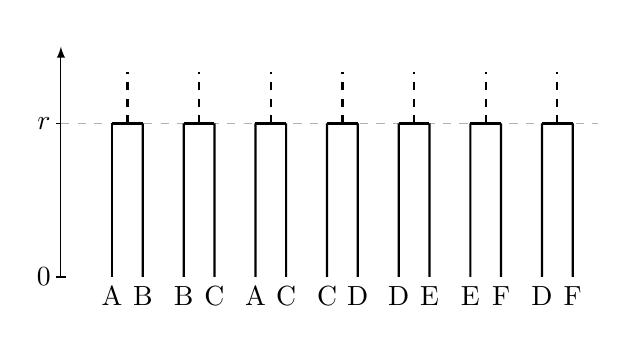
\begin{tikzpicture}[scale=0.65]
            
            % Hauteur de l'axe Y correspondant au niveau de fusion "r"
            \def\h{3.0}
            
            % Axe vertical pour localiser clairement la valeur r
            \draw[->, >=latex] (-1, 0) -- (-1, \h+1.5) node[above] {};
            \draw (-1.1, \h) -- (-0.9, \h) node[left=2pt] {$r$};
            \draw (-1.1, 0) -- (-0.9, 0) node[left=2pt] {$0$};
            
            % Ligne horizontale pointillée pour lier visuellement toutes les fusions à la hauteur r
            \draw[dashed, gray!60] (-1, \h) -- (9.5, \h);
            
            % Boucle générant la forêt des 7 fusions indépendantes
            % count=\i permet d'espacer mathématiquement chaque arbre sur l'axe X (0, 1.4, 2.8...)
            \foreach \L/\R [count=\i] in {A/B, B/C, A/C, C/D, D/E, E/F, D/F} {
                
                % Espacement horizontal entre les sous-dendrogrammes
                \pgfmathsetmacro{\x}{(\i-1)*1.4}
                
                % Coordonnées des feuilles
                \coordinate (L\i) at (\x, 0);
                \coordinate (R\i) at (\x+0.6, 0);
                
                % Affichage des lettres en bas
                \node[below] at (L\i) {\L};
                \node[below] at (R\i) {\R};
                
                % Lignes verticales montantes depuis les feuilles jusqu'au niveau r
                \draw[thick] (L\i) -- (\x, \h);
                \draw[thick] (R\i) -- (\x+0.6, \h);
                
                % Barre de fusion horizontale (le pont) au niveau r
                \draw[thick] (\x, \h) -- (\x+0.6, \h);
                
                % Pointillés verticaux montant depuis le milieu de la fusion
                % Ils indiquent que l'arbre complet continue de se construire au-dessus
                \draw[thick, dashed] (\x+0.3, \h) -- (\x+0.3, \h+1.0);
            }
            
        \end{tikzpicture}
        \caption{Fusions des sept segments au niveau $r$}
        \label{fig:foret_dendrogrammes}
    \end{subfigure}
    
    \caption{(Gauche) Nuage $\mathcal X$ repris de la \Fig~\ref{fig:nuage} avec les amas (en bleu) de forte densité $2$-NN au niveau $r' \gtrsim r$. (Droite) Dendrogramme en construction. Par convention, le multi-ensemble des feuilles apparaît au niveau $0$.}
    \label{fig:complexe_rprime}
\end{figure}


Pour $K=2$, les premiers amas de forte densité apparaissent au niveau $r$ (\emph{cf}. la \Fig~\ref{fig:intersections_rprime}). Ils sont au nombre de sept et en correspondance avec les sept segments de longueur $2r$ (\Fig~\ref{fig:foret_dendrogrammes}).


\begin{figure}[htbp]
    \centering
    
    % ---------------------------------------------------
    % SOUS-FIGURE (a) : Intersections au seuil r' exact
    % ---------------------------------------------------
    \begin{subfigure}[b]{0.45\textwidth}
        \centering
        \begin{tikzpicture}[scale=0.55]
            
            % r est la moitié du segment
            \def\r{1.5}
            
            % r' est calculé mathématiquement pour que les 3 cercles s'intersectent 
            % en 1 point central. Pour un triangle équilatéral de côté 2r, 
            % le rayon circonscrit est r' = 2r / sqrt(3).
            \pgfmathsetmacro{\rprime}{\r * 2 / sqrt(3)}
            
            % 1. Appel du template
            \templateNuage[\r]
            
            % 2. Dessin en arrière-plan
            \begin{scope}[on background layer]
                
                % Remplissage bleu foncé des intersections deux à deux
                % La superposition génère d'elle-même une zone un peu plus sombre
                % au centre où les 3 lentilles se chevauchent.
                \foreach \p/\q in {A/B, B/C, C/A, C/D, D/E, E/F, F/D} {
                    \begin{scope}
                        \clip (\p) circle (\rprime);
                        \fill[blue!60!black, opacity=0.4] (\q) circle (\rprime);
                    \end{scope}
                }
                
                % Tracé des 6 cercles de rayon r' (en pointillés gris)
                \foreach \P in {A,B,C,D,E,F} {
                    \draw[dashed, thick, gray!80] (\P) circle (\rprime);
                }
                
            \end{scope}
            
            % 3. Ajout des points rouges au centre des triangles 
            % Utilisation des coordonnées barycentriques de TikZ pour trouver le centre exact
            \fill[red] (barycentric cs:A=1,B=1,C=1) circle (3.5pt);
            \fill[red] (barycentric cs:D=1,E=1,F=1) circle (3.5pt);
            
            % 4. Flèche indiquant r' (orientée vers le haut-gauche)
            \draw[>=latex] (A) -- ++(135:\rprime) node[midway, sloped, above] {$r'$};
            
        \end{tikzpicture}
        \caption{$3$-intersection (rouge) pour $r' = \frac{2\sqrt{3}}{3}r$}
        \label{fig:intersections_rprime_exact}
    \end{subfigure}
    \hfill
    % ---------------------------------------------------
    % SOUS-FIGURE (b) : Dendrogrammes avec fusions à r et r'
    % ---------------------------------------------------
    \begin{subfigure}[b]{0.53\textwidth}
        \centering
        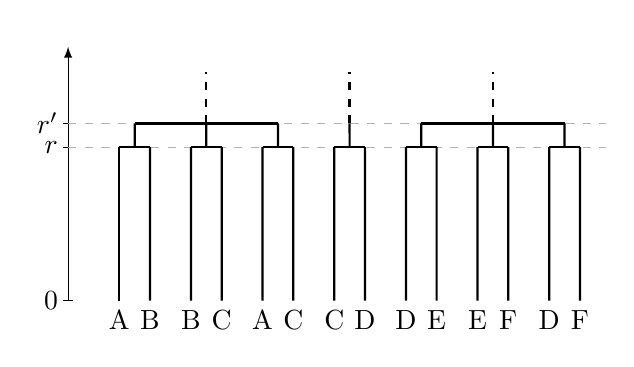
\begin{tikzpicture}[scale=0.65]
            
            % Hauteurs des niveaux de fusion
            \def\hr{3}      % Hauteur du niveau r
            \def\hrprime{3.46410161514} % Hauteur du niveau r'
            
            % Axe vertical des niveaux
            \draw[->, >=latex] (-1, 0) -- (-1, \hrprime+1.5) node[above] {};
            \draw (-1.1, \hr) -- (-0.9, \hr) node[left=2pt] {$r$};
            \draw (-1.1, \hrprime) -- (-0.9, \hrprime) node[left=2pt] {$r'$};
            \draw (-1.1, 0) -- (-0.9, 0) node[left=2pt] {$0$};
            
            % Lignes horizontales guides en pointillés
            \draw[dashed, gray!60] (-1, \hr) -- (9.5, \hr);
            \draw[dashed, gray!60] (-1, \hrprime) -- (9.5, \hrprime);
            
            % ==============================================
            % 1. BASE DU DENDROGRAMME : Fusions à r
            % ==============================================
            \foreach \L/\R [count=\i] in {A/B, B/C, A/C, C/D, D/E, E/F, D/F} {
                
                \pgfmathsetmacro{\x}{(\i-1)*1.4}
                \coordinate (L\i) at (\x, 0);
                \coordinate (R\i) at (\x+0.6, 0);
                
                % M\i représente le point central du pont de la fusion à r
                \coordinate (M\i) at (\x+0.3, \hr); 
                
                \node[below] at (L\i) {\L};
                \node[below] at (R\i) {\R};
                
                \draw[thick] (L\i) -- (\x, \hr);
                \draw[thick] (R\i) -- (\x+0.6, \hr);
                \draw[thick] (\x, \hr) -- (\x+0.6, \hr);
                
                % Prolongement vertical du tronc qui résulte de la fusion jusqu'à r'
                \draw[thick] (M\i) -- (\x+0.3, \hrprime);
            }
            
            % ==============================================
            % 2. ÉTAGE SUPÉRIEUR : Nouvelles fusions à r'
            % ==============================================
            
            % --- Fusion du triangle gauche (arêtes 1, 2, 3) ---
            % Leurs troncs arrivent aux abscisses 0.3, 1.7 et 3.1
            \draw[thick] (0.3, \hrprime) -- (3.1, \hrprime); % Pont horizontal qui relie les trois
            \draw[thick, dashed] (1.7, \hrprime) -- (1.7, \hrprime+1.0); % Le tronc commun en pointillés
            
            % --- Arête centrale C-D qui ne fusionne pas (arête 4) ---
            % Son tronc arrive à l'abscisse 4.5
            \draw[thick, dashed] (4.5, \hrprime) -- (4.5, \hrprime+1.0); % Continue de monter seule
            
            % --- Fusion du triangle droit (arêtes 5, 6, 7) ---
            % Leurs troncs arrivent aux abscisses 5.9, 7.3 et 8.7
            \draw[thick] (5.9, \hrprime) -- (8.7, \hrprime); % Pont horizontal qui relie les trois
            \draw[thick, dashed] (7.3, \hrprime) -- (7.3, \hrprime+1.0); % Le tronc commun en pointillés
            
        \end{tikzpicture}
        \caption{Fusions de dimension supérieure à $r'$}
        \label{fig:fusion_rprime}
    \end{subfigure}
    
    \caption{(Gauche) Évolution des amas de forte densité $2$-NN au niveau $r' = \frac{2\sqrt{3}}{3}r$ : on voit apparaître des fusions de $2$-intersections de boules au moyen de $3$-intersections (le point de contact de la fusion est repéré en rouge). (Droite) : Évolution du dendrogramme avec les fusions opérées au niveau $r'$.}
    \label{fig:complexe_rprime_exact}
\end{figure}

Au niveau $r' = \frac{2\sqrt{3}}{3}r$, des $3$-intersections de boules apparaissent, fusionnant certains amas de forte densité. Voir la \Fig~\ref{fig:complexe_rprime_exact} pour plus de détails.



\begin{figure}[htbp]
    \centering
    
    % ---------------------------------------------------
    % SOUS-FIGURE (a) : Intersections au seuil r'' = AD/2
    % ---------------------------------------------------
    \begin{subfigure}[b]{0.48\textwidth}
        \centering
        \begin{tikzpicture}[scale=0.45]
            
            \def\r{1.5}
            
            % r'' = AD/2. La formule mathématique exacte :
            \pgfmathsetmacro{\rsecond}{\r * sqrt(2 + sqrt(3))}
            
            % 1. Appel du template modifié au premier plan
            \templateNuage[\r]
            
            % 2. Dessin des intersections sous le graphe (arrière-plan)
            \begin{scope}[on background layer]
                
                % -- 2-INTERSECTIONS (Bleu foncé surfacique) --
                \foreach \p/\q in {A/B, B/C, C/A, C/D, D/E, E/F, F/D} {
                    \begin{scope}
                        \clip (\p) circle (\rsecond);
                        \fill[blue!60!black, opacity=0.25] (\q) circle (\rsecond);
                    \end{scope}
                }
                
                % -- 3-INTERSECTIONS (Rouge pur) --
                % Triangle gauche (A, B, C)
                \begin{scope}
                    \clip (A) circle (\rsecond);
                    \clip (B) circle (\rsecond);
                    \clip (C) circle (\rsecond);
                    % On efface le bleu sous-jacent avec du blanc, puis on remplit en rouge
                    \fill[white] (-10,-10) rectangle (10,10); 
                    \fill[red, opacity=0.6] (-10,-10) rectangle (10,10);
                \end{scope}
                
                % Triangle droit (D, E, F)
                \begin{scope}
                    \clip (D) circle (\rsecond);
                    \clip (E) circle (\rsecond);
                    \clip (F) circle (\rsecond);
                    \fill[white] (-10,-10) rectangle (10,10); 
                    \fill[red, opacity=0.6] (-10,-10) rectangle (10,10);
                \end{scope}
                
                % Tracé des 6 grands cercles originaux (pointillés gris)
                \foreach \P in {A,B,C,D,E,F} {
                    \draw[dashed, thick, gray!60] (\P) circle (\rsecond);
                }
                
            \end{scope}
            
            % 3. Ajout didactique des 4 points de tangence simultanés (en rouge)
            % Calculés par TikZ avec une précision absolue au milieu des segments croisés
            \fill[red] ($ (A)!0.5!(D) $) circle (3.5pt); % Tangence A-D (Haut côté C)
            \fill[red] ($ (C)!0.5!(E) $) circle (3.5pt); % Tangence C-E (Haut côté D)
            \fill[red] ($ (B)!0.5!(D) $) circle (3.5pt); % Tangence B-D (Bas côté C)
            \fill[red] ($ (C)!0.5!(F) $) circle (3.5pt); % Tangence C-F (Bas côté D)
            
            % Flèche indiquant le rayon r'' (dirigée vers l'extérieur pour ne rien masquer)
            \draw[>=latex] (A) -- ++(135:\rsecond) node[midway, sloped, above=1pt] {$r''$};
            
        \end{tikzpicture}
        \caption{Connexité globale atteinte pour $r''=AD/2$}
        \label{fig:intersections_rsecond}
    \end{subfigure}
    \hfill
    % ---------------------------------------------------
    % SOUS-FIGURE (b) : Dendrogramme final complet
    % ---------------------------------------------------
    \begin{subfigure}[b]{0.51\textwidth}
        \centering
        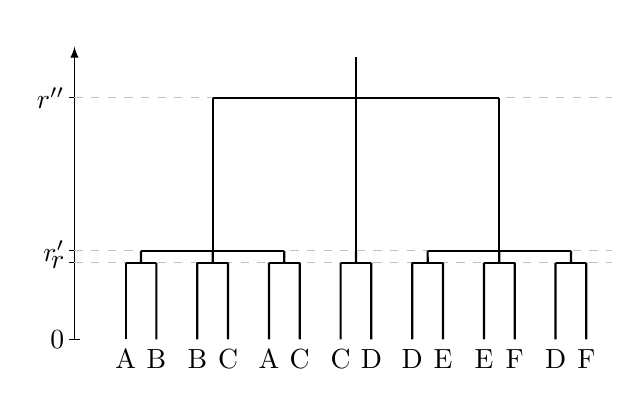
\begin{tikzpicture}[scale=0.65]
            
            % Hauteurs successives des 3 niveaux de fusion
            \def\hr{1.5}       % Niveau r
            \def\hrprime{1.732}  % Niveau r' 1.5 * 2/3 \sqrt{3}
            \def\hrsecond{4.72} % Niveau r'' 1.5*(\sqrt{3}+\sqrt{2})
            %\pgfmathsetmacro{\rsecond}{\r * sqrt(2 + sqrt(3))}
            
            % Axe vertical
            \draw[->, >=latex] (-1, 0) -- (-1, \hrsecond+1.0) node[above] {};
            \draw (-1.1, \hr) -- (-0.9, \hr) node[left=2pt] {$r$};
            \draw (-1.1, \hrprime) -- (-0.9, \hrprime) node[left=2pt] {$r'$};
            \draw (-1.1, \hrsecond) -- (-0.9, \hrsecond) node[left=2pt] {$r''$};
            \draw (-1.1, 0) -- (-0.9, 0) node[left=2pt] {$0$};
            
            % Lignes guides horizontales
            \draw[dashed, gray!50] (-1, \hr) -- (9.5, \hr);
            \draw[dashed, gray!50] (-1, \hrprime) -- (9.5, \hrprime);
            \draw[dashed, gray!50] (-1, \hrsecond) -- (9.5, \hrsecond);
            
            % ==============================================
            % NIVEAU 1 : Fusions initiales à r
            % ==============================================
            \foreach \L/\R [count=\i] in {A/B, B/C, A/C, C/D, D/E, E/F, D/F} {
                \pgfmathsetmacro{\x}{(\i-1)*1.4}
                \coordinate (L\i) at (\x, 0);
                \coordinate (R\i) at (\x+0.6, 0);
                \coordinate (M\i) at (\x+0.3, \hr); 
                
                \node[below] at (L\i) {\L};
                \node[below] at (R\i) {\R};
                
                \draw[thick] (L\i) -- (\x, \hr);
                \draw[thick] (R\i) -- (\x+0.6, \hr);
                \draw[thick] (\x, \hr) -- (\x+0.6, \hr);
                
                % Les 7 troncs montent jusqu'au niveau r'
                \draw[thick] (M\i) -- (\x+0.3, \hrprime);
            }
            
            % ==============================================
            % NIVEAU 2 : Fusions des sous-composantes à r'
            % ==============================================
            % Tronc gauche (fusion du triangle ABC)
            \draw[thick] (0.3, \hrprime) -- (3.1, \hrprime);
            \draw[thick] (1.7, \hrprime) -- (1.7, \hrsecond);
            
            % Tronc droit (fusion du triangle DEF)
            \draw[thick] (5.9, \hrprime) -- (8.7, \hrprime);
            \draw[thick] (7.3, \hrprime) -- (7.3, \hrsecond);
            
            % Arête centrale 4 (C/D) qui traverse r' sans fusionner
            \draw[thick] (4.5, \hrprime) -- (4.5, \hrsecond); 
            
            % ==============================================
            % NIVEAU 3 : Fusion finale globale à r''
            % ==============================================
            % On unifie le tronc gauche (x=1.7), le tronc central (x=4.5) et le tronc droit (x=7.3)
            \draw[thick] (1.7, \hrsecond) -- (7.3, \hrsecond);
            
            % Racine finale du dendrogramme (Single-Linkage) en trait PLEIN
            \draw[thick] (4.5, \hrsecond) -- (4.5, \hrsecond+0.8);
            
        \end{tikzpicture}
        \caption{Clôture du dendrogramme à $r''$}
        \label{fig:fusion_rsecond}
    \end{subfigure}
    
    \caption{Clôture de la hiérarchie $2$-NN au niveau $r'' = AD/2$. À ce rayon critique, l'apparition simultanée des quatre points de tangence (points rouges) relient les trois amas de forte densité.}
    \label{fig:complexe_rsecond}
\end{figure}

Enfin, au niveau $r''= \frac{AD}{2}$, des jonctions apparaissent entre les trois amas de forte densité du niveau $r'$, clôturant ainsi le dendrogramme. Voir la \Fig~\ref{fig:complexe_rsecond}.

Comme déjà esquissé dans la première partie, l'on s'aperçoit que pour rendre compte des $K \ge 2$ plus proches voisins, il va être nécessaire de relâcher l'hypothèse d'un clustering vu comme une \emph{partition} sur les données $\mathcal X$.
Les interactions d'ordre supérieur (ici des arêtes connectées entre elles au moyen de triangles\footnote{C'est pourquoi le seuil de connexion global sur notre exemple est  $r'' = AD/2$ : à ce niveau, le triangle ACD apparaît connectant les arêtes AC et CD.}) s'avèrent nécessaires.


\section{Du graphe géométrique au complexe de \v Cech : les $K$-polyèdres}
\label{sec:KPolyedres}

Pour généraliser correctement le Single-Linkage, nous prenons comme point de départ l'axe (développé dans la partie~I) d'analyse persistante sur des \emph{graphes géométriques} (\Def[def:dendrogramme_gg]).
%Le point de vue sur le Single-Linkage développé dans la partie~I que nous reprenons comme point de départ est celui d'une analyse persistante sur des graphes géométriques (\Def~\ref{def:dendrogramme_gg}). 
La généralisation naturelle consiste à remplacer les graphes par des hypergraphes\footnote{Un graphe est la donnée d'un ensemble de sommets noté $V$ (pour \emph{vertices} en anglais) et d'un ensemble de relation binaires entre ces sommets, les arêtes $E$ (\emph{edges} en anglais). Dans le cas d'un \emph{hyper}graphe, les arêtes deviennent des hyper-arêtes, c'est-à-dire qu'elles ne sont plus nécessairement binaires mais peuvent encoder des relation d'ordre supérieur : des triangles, des tétraèdres, \emph{etc}.}.
Plus précisément, une sous-famille des hypergraphes va nous servir au cours de ce manuscrit : les complexes simpliciaux \cite{Munkres}. Un complexe simplicial est un hypergraphe pour lequel la présence d'une hyper-arête entraîne la présence de toutes les sous-hyper-arêtes. Par exemple, la présence d'un tétraèdre entraîne la présence de ses quatre ``facettes'' (triangles), de ses quatre arêtes (et bien-sûr des quatre sommets, que l'on peut voir comme des hyper-arêtes d'ordre $0$).

Il devient alors possible de remplacer les composantes connexes ordinaires par une ``connectivité'' d'ordre supérieur.

\subsection{Le complexe de \v Cech}

\begin{Definition}{Complexe de \v Cech \cite{Cech1932, Munkres, BoissonnatChazalYvinec}}{cech_complexe}
Soit $\X\subset \mathbb R^p$ un nuage fini et $r\ge 0$. Le \emph{complexe de \v Cech} de rayon $r$ est le complexe simplicial
\[
\boxed{
    \check C(\X,r) \eqdef \left\{\sigma\subseteq \X \ \middle|\  \bigcap_{x\in \sigma}\overline B(x,r)\neq \varnothing \right\}.
    }
\]
Autrement dit, un ensemble fini $\sigma\subseteq \X$ est un simplexe de $\check C(\X,r)$ si et seulement s'il existe un point $y\in\mathbb R^p$ situé à distance au plus $r$ de tous les sommets de $\sigma$, \emph{i.e.}
\[
\sigma \subset \overline B(y,r).
\]
\end{Definition}

%\textcolor{red}{Parler aussi des complexes de Vietoris--Rips ? notamment pour les approximations dans le cas de figure non euclidien ? Ou bien y consacrer un court chapitre ? }

\Remarque{Le $1$-squelette de $\check C(\X,r)$ n'est autre que le graphe géométrique $\mathcal G(\X,r)$ introduit au chapitre \ref{chap:single-linkage_trois_vues} : une arête $\{x,x'\}$ apparaît exactement lorsque $\overline B(x,r)\cap \overline B(x',r)\neq\varnothing$, c'est-à-dire lorsque $\norme{x-x'}\le 2r$.}

Plus généralement, un $K$-simplexe de $\check C(\X,r)$ encode une interaction entre $K+1$ points qui peuvent être simultanément vus depuis une même boule de rayon $r$. C'est précisément ce type d'information sur la densité locale qui manque au Single-Linkage et qui est la source de l'effet de chaînage.

\subsection{Les $K$-polyèdres}

\begin{Definition}{Graphe des $(K-1)$-simplexes et $K$-polyèdres}{k_polyedres}
Soit $K\in \IntervalleEntiers{1,|\X|}$ et $r\ge 0$. On note $\check C_{K-1}(\X,r)$ l'ensemble des simplexes de dimension $K-1$ du complexe de \v Cech $\check C(\mathcal X, r)$.

On leur associe le graphe
\[
    \Gamma_K(\X,r)
\]
dont les sommets sont les éléments de $\check C_{K-1}(\X,r)$, deux sommets $\sigma$ et $\tau$ étant reliés dès que $\sigma\cup\tau$ est encore un simplexe de $\check C(\X,r)$.

Un \emph{$K$-polyèdre} de $\check C(\X,r)$ est alors l'ensemble des points de $\X$ apparaissant dans une composante connexe de $\Gamma_K(\X,r)$.
\end{Definition}

\Remarque{Cette définition prolonge la notion usuelle de composante connexe, qu'on retrouve pour $K=1$ : les sommets de $\Gamma_1(\X,r)$ sont les points de $\X$ et ses arêtes sont celles telles que $\norme{x-x'} \le 2r$ ; les $1$-polyèdres sont donc les composantes connexes ordinaires du graphe géométrique $\mathcal G(\mathcal X,r) = \Gamma_1(\X,r)$. Pour $K=2$, les sommets de $\Gamma_2(\X,r)$ sont les arêtes de $\check C(\X,r)$ et deux arêtes partageant un sommet deviennent adjacentes dès que le triangle qu'elles forment apparaît.
%\textcolor{red}{Illustrer ? ou est-ce déjà assez clair ?}
Cette façon de connecter entre eux des simplexes (vu comme des cliques sur un graphe) au moyen d'une clique plus grande est appelée \emph{clique percolation} \cite{KCliquePercolation}. Pour le cas plus général des complexes simpliciaux, \textsc{Atkin} avait déjà défini en 1972 ce qu'il nommait la $q$-\emph{connectivity} \cite{Atkin1972}. Aujourd'hui, l'usage serait plutôt d'employer le terme \emph{(up) face percolation} \cite{HirschValesin2025}.}

\begin{Definition}{HGP-Clusterer (HGP pour Hypergraphe-Percol')}{hgp_clusterer}
Pour $K\in \IntervalleEntiers{1,|\X|}$, on définit \emph{Hypergraphe-Percol'} (acronyme : HGP) par
\[
\boxed{
    \theta^{\mathrm{HGP}}_K(r) \eqdef \left\{\text{$K$-polyèdres de } \check C(\X,r)\right\},
    \qquad \text{ pour tout }r\ge 0.
    }
\]
Autrement dit, HGP-Clusterer observe l'évolution des $K$-polyèdres au fil de la filtration du complexe de \v Cech.
\end{Definition}

\Remarque{La filtration $r\mapsto \check C(\X,r)$ est croissante, donc le graphe $\Gamma_K(\X,r)$ l'est aussi. Les $K$-polyèdres ne peuvent ainsi que croître et fusionner lorsque $r$ augmente. Pour $K=1$, on retrouve exactement le Single-Linkage de la partie~I.}

\begin{figure}[!ht]
    \centering
    \begin{subfigure}[b]{0.48\textwidth}
        \centering
        \begin{tikzpicture}[scale=0.55]
            \def\r{1.5}
            \pgfmathsetmacro{\rprime}{2*sqrt(3)/3*\r}
            \pgfmathsetmacro{\h}{\r*sqrt(3)}

            \coordinate (C) at (-\r, 0);
            \coordinate (D) at (\r, 0);
            \coordinate (A) at (-\r-\h, \r);
            \coordinate (B) at (-\r-\h, -\r);
            \coordinate (E) at (\r+\h, \r);
            \coordinate (F) at (\r+\h, -\r);

            \begin{scope}[on background layer]
                \fill[blue!18] (A) -- (B) -- (C) -- cycle;
                \fill[red!18]  (D) -- (E) -- (F) -- cycle;
            \end{scope}

            \templateNuage[\r]

            \foreach \P in {A,B,C,D,E,F} {
                \draw[dashed, gray!70] (\P) circle (\rprime);
            }

            \node[blue!70!black] at (-4.2,2.6) {$ABC$};
            \node[red!70!black]  at (4.2,2.6) {$DEF$};
            \node[above=4pt] at ($(C)!0.5!(D)$) {$CD$};
        \end{tikzpicture}
        \caption{Complexe de \v Cech pour $K=2$}
        \label{fig:chap2_cech_exemple}
    \end{subfigure}
    \hfill
    \begin{subfigure}[b]{0.48\textwidth}
        \centering
        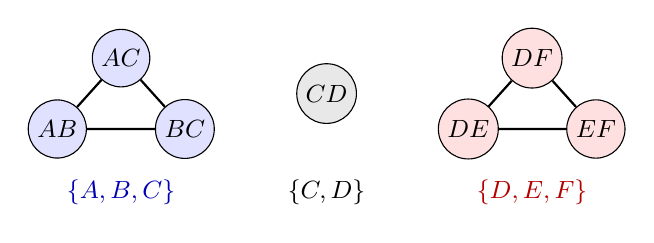
\begin{tikzpicture}[scale=0.9, every node/.style={font=\small}]
            \node[circle, draw, fill=blue!12, inner sep=2pt] (ab) at (0,1.0) {$AB$};
            \node[circle, draw, fill=blue!12, inner sep=2pt] (ac) at (0.9,2.0) {$AC$};
            \node[circle, draw, fill=blue!12, inner sep=2pt] (bc) at (1.8,1.0) {$BC$};
            \draw[thick] (ab)--(ac)--(bc)--(ab);

            \node[circle, draw, fill=gray!18, inner sep=2pt] (cd) at (3.8,1.5) {$CD$};

            \node[circle, draw, fill=red!12, inner sep=2pt] (de) at (5.8,1.0) {$DE$};
            \node[circle, draw, fill=red!12, inner sep=2pt] (df) at (6.7,2.0) {$DF$};
            \node[circle, draw, fill=red!12, inner sep=2pt] (ef) at (7.6,1.0) {$EF$};
            \draw[thick] (de)--(df)--(ef)--(de);

            \node[blue!70!black] at (0.9,0.1) {$\{A,B,C\}$};
            \node at (3.8,0.1) {$\{C,D\}$};
            \node[red!70!black] at (6.7,0.1) {$\{D,E,F\}$};
        \end{tikzpicture}
        \caption{Le graphe $\Gamma_2(\X,r)$ associé}
        \label{fig:chap2_gamma2_exemple}
    \end{subfigure}
    \caption{Exemple de $2$-polyèdres sur la configuration à six points de l'exemple en \S~\ref{sec:exemple_introductif}. Au rayon $r'=\frac{2\sqrt 3}{3}r$, le complexe de \v Cech contient deux triangles $ABC$ et $DEF$ ainsi que l'arête $CD$. Les composantes connexes du graphe $\Gamma_2(\X,r')$ donnent alors trois $2$-polyèdres, à savoir $\{A,B,C\}$, $\{C,D\}$ et $\{D,E,F\}$. On voit déjà apparaître le phénomène essentiel : pour $K\ge 2$, les polyèdres peuvent se recouvrir.}
    \label{fig:chap2_exemple_kpolyedres}
\end{figure}

La \Fig~\ref{fig:chap2_exemple_kpolyedres} illustre la différence de nature entre la connexité ordinaire et la connexité d'ordre supérieur. Dans le cas $K=2$, ce ne sont plus les points qui percolent directement, mais les arêtes, recollées entre elles par des triangles.

\section{$K$-polyèdres de \v Cech et amas discrets de forte densité $K$-NN}
\label{sec:correspondance_KPolydres_KNN}


Au cours de la première partie, nous avons introduit l'estimateur $K$-NN de densité des $K$ plus proches voisins (\Def[def:K-NN]) et les amas \emph{discrets} de forte densité qui lui sont associés (\Def[def:HDC_discret]). Rappelons qu'à rayon $r>0$ fixé, le niveau supérieur s'écrit
\[
    L_K(r) \eqdef \left\{ y\in\mathbb R^p \ \middle|\ \module{\overline B(y,r)\cap \X}\ge K \right\},
\]
et que les clusters ({continus}) sont les composantes connexes de $L_K(r)$. Les clusters \emph{discrets} sont les ensembles de points \emph{couverts} (c'est-à-dire à moins de $r$) par ces clusters continues (ils participent \emph{via} $K$-NN à l'existence du cluster continu).

Le résultat central de ce chapitre (\Th~\ref{th:cech_kpolyedres_knn} ci-dessous) est le suivant : les $K$-polyèdres du complexe de \v Cech identifient exactement les amas discrets de forte densité $K$-NN.

\subsection{Les régions témoins d'un simplexe}

Pour tout $(K-1)$-simplexe $\sigma\in \check C_{K-1}(\X,r)$, introduisons l'ensemble
\[
    T_r(\sigma) \eqdef \bigcap_{x\in \sigma} \overline B(x,r).
\]
Nous l'appellerons la \emph{région témoin} du simplex $\sigma$ au niveau $r$. Par construction, $T_r(\sigma)$ est une intersection finie de boules fermées : c'est donc un compact convexe, en particulier connexe.
L'idée de la preuve du \Th~\ref{th:cech_kpolyedres_knn} est simple : le niveau supérieur $L_K(r)$ est exactement l'union de ces régions témoins pour tous les $(K-1)$-simplexes de $\check C(\mathcal X, r)$, et le graphe $\Gamma_K(\X,r)$ n'est rien d'autre que leur graphe d'intersection.

\begin{Theoreme}{$K$-polyèdres de \v Cech $\equiv$ amas discrets de forte densité $K$-NN}{cech_kpolyedres_knn}
Soit $\X\subset \mathbb R^p$ un nuage fini de taille $n$, $K\in \IntervalleEntiers{1,n}$ et $r>0$. Alors les $K$-polyèdres du complexe de \v Cech $\check C(\X,r)$ sont en correspondance avec les amas discrets de forte densité
\[
    H^{\mathrm{discrets}}_{\widehat f_K}(r).
\]

Plus précisément, si $C$ est une composante connexe de
\[
    L_K(r)=\left\{ y\in\mathbb R^p \ \middle|\ |\overline B(y,r)\cap \X|\ge K \right\}
\]
et si $P_C$ désigne le $K$-polyèdre correspondant, alors
\[
    P_C = C^{\mathrm{discret}} = \left\{ x\in \X \ \middle|\ \exists y\in C,\ \norme{x-y}\le r \right\}.
\]
En particulier,
\[
\boxed{
    \theta^{\mathrm{HGP}}_K(r) = H^{\mathrm{discrets}}_{\widehat f_K}(r)
    \qquad\text{pour tout } r\ge 0,
    }
\]
et $\theta^{\mathrm{HGP}}_1 $ coïncide avec le Single-Linkage ($\theta^{\mathrm{HGP}}_1 = \theta^\sim$, voir \Def[def:dendrogramme_gg]).
\end{Theoreme}

\begin{Preuve}[{Preuve du \Th~\ref{th:cech_kpolyedres_knn}}]
% Pour tout $(K-1)$-simplex $\sigma\in \check C_{K-1}(\X,r)$, posons
% \[
%     T_r(\sigma) \eqdef \bigcap_{x\in \sigma}\overline B(x,r).
% \]
% Les ensembles $T_r(\sigma)$ sont des compacts convexes.
Le niveau supérieur $L_K(r)$ est recouvert par les régions témoins : on a l'égalité
\[
    L_K(r)=\bigcup_{\sigma\in\check C_{K-1}(\X,r)} T_r(\sigma).
\]
En effet, si $y\in L_K(r)$, alors la boule $\overline B(y,r)$ contient au moins $K$ points de $\X$. Si l'on en choisit $K$, on obtient un $(K-1)$-simplexe $\sigma$ tel que $y\in T_r(\sigma)$. Réciproquement, si $y\in T_r(\sigma)$ pour un simplex $\sigma$ de cardinal $K$, alors $\overline B(y,r)$ contient les $K$ sommets de $\sigma$, donc $y\in L_K(r)$.

Le graphe $\Gamma_K(\X,r)$ est le graphe d'intersection de ce recouvrement.
Pour deux $(K-1)$-simplexes $\sigma$ et $\tau$, on a
\[
    T_r(\sigma)\cap T_r(\tau)\neq \varnothing
    \iff \bigcap_{x\in \sigma\cup\tau}\overline B(x,r)\neq \varnothing
    \iff \sigma\cup\tau\in \check C(\X,r).
\]
Ce qui est précisément la règle d'adjacence qui définit $\Gamma_K(\X,r)$.

Comme la famille $\{T_r(\sigma)\}_{\sigma\in\check C_{K-1}(\X,r)}$ est finie et formée de compacts connexes, les composantes connexes de son union correspondent exactement aux unions des régions témoins de chacune des composantes connexes du graphe d'intersection. 
Il existe ainsi une bijection naturelle entre les composantes connexes de $L_K(r)$ et les $K$-polyèdres de $\check C(\X,r)$.

Scrutons à présent le cluster discret associé à une région connexe.
Soit $C$ une composante connexe de $L_K(r)$, $P_C$ le $K$-polyèdre qui lui correspond et $C^{\mathrm{discret}}$ le cluster discret associé.

Montrons d'abord l'inclusion $P_C\subseteq C^{\mathrm{discret}}$. Si $x\in P_C$, alors $x$ appartient à un $(K-1)$-simplex $\sigma$ tel que $T_r(\sigma)\subseteq C$. Choisissons $y\in T_r(\sigma)$. Comme $x$ est l'un des sommets de $\sigma$, on a $\norme{x-y}\le r$. Le point $x$ est donc couvert par $C$, d'où $x\in C^{\mathrm{discret}}$.

Réciproquement, soit $x\in C^{\mathrm{discret}}$. Par définition, il existe $y\in C$ tel que $\norme{x-y}\le r$. Puisque $y\in L_K(r)$, l'ensemble $\overline B(y,r)\cap \X$ contient au moins $K$ points et il contient en particulier $x$. On peut donc choisir $K-1$ autres points $x_2,\ldots,x_K\in \overline B(y,r)\cap \X$ et former le simplexe
\[
    \sigma = \{x,x_2,\ldots,x_K\}\in \check C_{K-1}(\X,r).
\]
Comme $y\in T_r(\sigma)\subseteq C$, le simplex $\sigma$ appartient à la composante de $\Gamma_K(\X,r)$ associée à $C$. L'un de ses sommets étant $x$, on obtient $x\in P_C$.

On a donc bien $P_C=C^{\mathrm{discret}}$, ce qui conclut la preuve.
\end{Preuve}

\Remarques{Dans le cas $K=1$, les régions témoins sont simplement les boules $\overline B(x,r)$ centrées sur les données. Le graphe d'intersection redevient alors le graphe géométrique, et le \Th~\ref{th:cech_kpolyedres_knn} retrouve exactement la synthèse obtenue à la fin du chapitre \ref{chap:single-linkage_trois_vues}.
\textcolor{red}{$K=2$}}

%\textcolor{red}{Besoin d'une autre illustration pour le graphe d'intersection des régions témoin ?}

\Synthese{Ce chapitre a d'abord permis, au travers d'un exemple, de montrer les limites des algorithmes actuels comme le Robust Single-Linkage et (H)DBSCAN\footnote{L'on aurait pu aussi citer les auteurs de \cite{GeneralizedSL}, qui construisent un graphe géométrique sur les données puis échantillonnent la densité le long de ses arêtes.} et de donner l'intuition de l'algorithme que nous proposons. 

Il généralise ensuite exactement les deux premières vues du Single-Linkage :
\begin{enumerate}
    \item \textbf{Modèle géométrique d'analyse persistante.} Le graphe géométrique est remplacé par le complexe de \v Cech et la composante connexe par un $K$-polyèdre.
    \item \textbf{Modèle statistique de \textsc{Hartigan}}. Le \Th~\ref{th:cech_kpolyedres_knn} montre que cette construction coïncide niveau par niveau avec les amas discrets de forte densité $H^{\mathrm{discrets}}_{\widehat f_K}(r)$.
\end{enumerate}

La définition proposée dans ce chapitre de HGP-Clusterer (\Def[def:hgp_clusterer]) reste bien-sûr toute théorique (comme l'était la définition du Single-Linkage en \Def[def:dendrogramme_gg], recourant à des graphes géométriques).

Il reste au cours des chapitres suivants à retrouver le troisième volet du triptyque : définir HGP-Clusterer au moyen d'un objet combinatoire (beaucoup) plus mince jouant le rôle de l'\textbf{arbre minimum couvrant}. C'est sur cet arbre couvrant généralisé qu'est calculée en pratique la hiérarchie $K$-NN des amas de forte densité.}